\documentclass{ML}

% 姓名,学号
\infoauthor{朱明彦}{1160300314}

% 课程类型,实验名称
\infoexp{课程类型}{实验二}

\infoschool{计算机学院}{高宏}

\begin{document}
\maketitle

% \tableofcontents
\newpage

\begin{center}
    \textbf{\zihao{3} 实验二 \ 使用高级语言操作MySQL数据库}
\end{center}

对于 3.1,粘贴 9 条 sql 语句的核心高级语言函数代码以及相应的查询结果,
作为评分标准。先进行 3.2-3.5 的操作练习,结果无需截图。

\section{实验目的}
学会使用高级语言访问 MySQL 数据库,并进行查询。
\section{实验环境}
\begin{itemize}
    \item Ubuntu 16.04.5
    \item MySQL Ver 14.14 Distrib 5.7.25
    \item Java version 1.8.0\_181
    \item IntelliJ IDEA Ultimate 2018.3.5
\end{itemize}
\section{实验过程及结果}
\begin{enumerate}
    \item \begin{minted}{Java}
    String PARA_PNO = "%PNO%";
    String query = "SELECT ESSN FROM WORKS_ON WHERE PNO = \"" + PARA_PNO + "\"";
    System.out.println("Query " + count);
    System.out.println("Please input pno:");
    String pno = cin.nextLine();
    query = query.replace(PARA_PNO, pno);
    resultSet = statement.executeQuery(query);
    while (resultSet.next())
        System.out.println(resultSet.getNString("ESSN"));
    \end{minted}
    实验结果如下:
    \begin{figure}[htb]
        \centering
        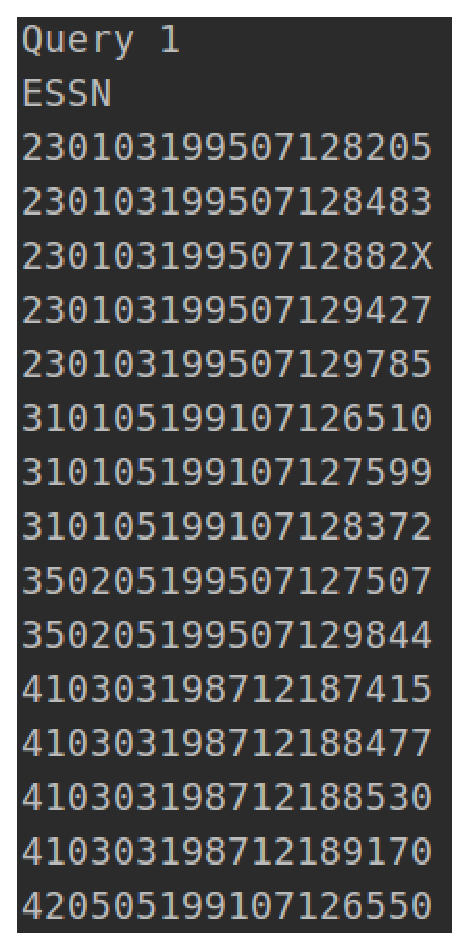
\includegraphics[scale=0.5, bb=0 0 217 485]{media/3.1.eps}
    \end{figure}
    % \begin{minted}
        
    % \end{minted}
\end{enumerate}
\section{实验心得}

% \appendix

% \section{源代码}
% \section{参考文献}
% \begin{thebibliography}{20}
%     % \bibitem{employee_name} 中国最常见名字前50名, \texttt{https://www.sohu.com/a/164406113\_367620}
%     \bibitem{employee_id} 身份证号在线生成器, \texttt{https://www.tinysoft.org/}
% \end{thebibliography}

\end{document}
